\subsection{What Constitutes Reception?}
\begin{frame}[t]{What Constitutes Reception?}
\small
\begin{block}{}
\textsl{Reception} happens when one planet (A) is in the domicile or exaltation of another planet (B) whom it aspects or conjuncts. The aspect (or conjunction) from planet \textsl{A} must \textsl{perfect} (become exact)  before planet \textsl{B} moves into another sign or a third planet (C) intercedes by completing its own aspect or conjunction with planet \textsl{B}.
\end{block}

While Masha'Allah appears to have been the first to begin categorizing and explaining the way reception, applications, and separations indicate outcomes Sahl ibn Bishr al-Israili (786-845) was the first I could find that defined 16 distinct modes of the "perfection and destruction of things". These were also listed and amplified by  Abu Ma'shar (787-886),  ibn Ezra (1089-1164), and much later they are described in Guido Bonatti's \textsl{Liber Astronomaie}.

Examples from all the earlier authors may be used to name and describe the various ways in which reception, or prohibition, can occur. The referenced texts are:
\begin{itemize}
\small
\item \textsl{The Introduction to the Science of the Judgments of the Stars} by Sahl ibn Bisher trans. James Holden, AFA, 2008

\item \textsl{The Abbreviation of the Introduction to Astrology} by Abu Ma'shar trans. Charles Burnett, ARHAT, 2nd. printing, 2000

\item \textsl{Ibn Ezra: The Beginning of Wisdom} trans. Meira Epstein, ARHAT, 1998
\end{itemize}

\end{frame}
% -------------------------------------------------------------------
\begin{frame}[t]{What Constitutes Reception - Perfect Reception}
\vspace{0.1cm}
\begin{columns}[T, onlytextwidth]
\column{0.5\textwidth}
An example of \textbf{perfect reception} (according to Sahl\footnotemark[1]) is a planet applying to the domicile or exaltation ruler of the sign it occupies. \\
\vspace{0.2cm}
\textbf{Example: \Moon\ in \Aries\ $\Rightarrow$ \Mars\ or \Sun} 
\ul
\vspace{0.2cm}
\Moon\ in \Aries\ applying to either of \\
\Mars\ (domicile ruler) or \\
\Sun\ (exaltation ruler) \\
\vspace{0.2cm}
\Mars\ or the \Sun\ can be in any sign; they receive the \Moon\ because she is in \Aries\ which \Mars\ rules by domicile and the \Sun\ by exaltation.
\column{0.5\textwidth}
\vspace{-0.5cm}

\begin{center}
{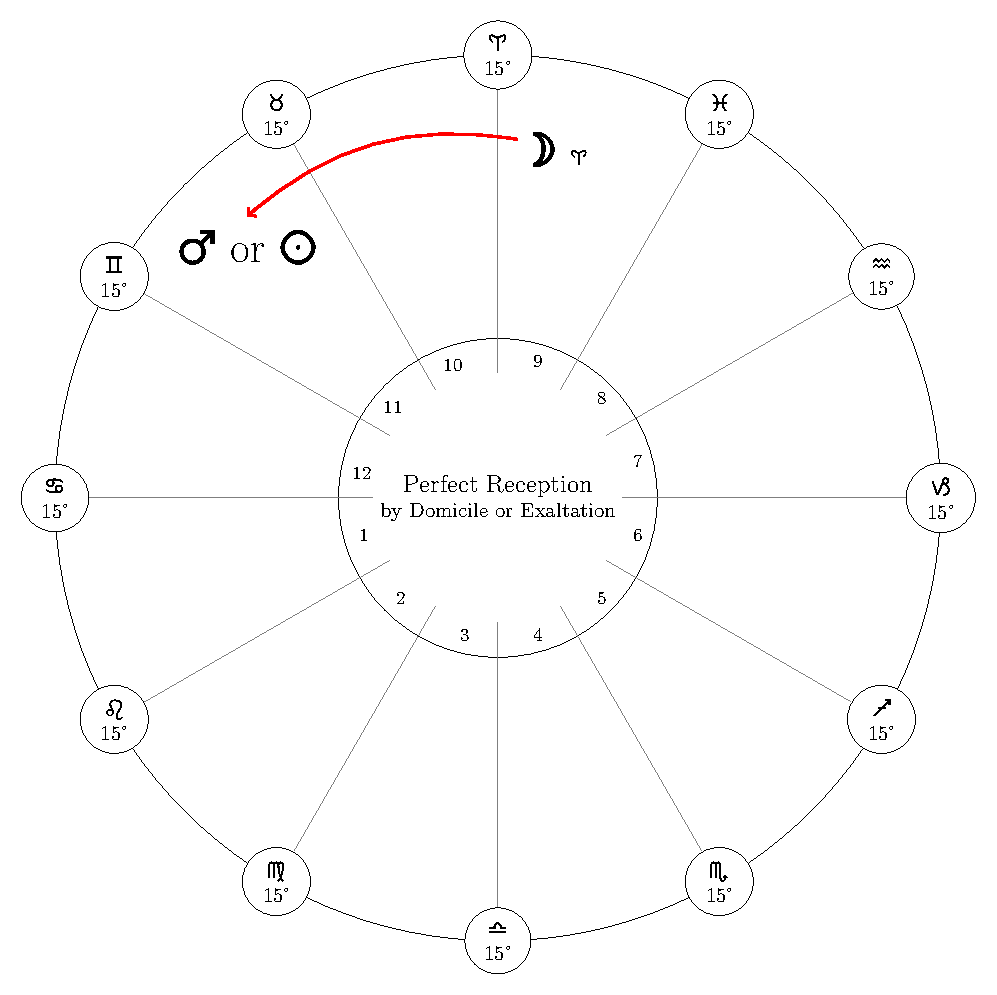
\includegraphics[width=0.8\textwidth]{charts/01-perfect-reception}} \\
\end{center}

\end{columns}
\vspace{0.2cm}
\footnotetext[1]{Sahl, p.18}
\end{frame}
% ----------------------------------------------------
\begin{frame}[t]{What Constitutes Reception - A Weaker Reception}
\begin{columns}[T, onlytextwidth]
\column{0.5\textwidth}
A planet in its own domicile or exaltation applying to another planet is said by Abu Ma'shar to \textsl{"push [its] power"} to the other planet.\footnotemark[1] Ibn Ezra calls it \textsl{"conferring influence"}.\footnotemark[2]This too is a form of reception but it is considered weaker than perfect reception.\\
\vspace{0.2cm}
\textbf{Example:} \Mars\ or \Sun\ in \Aries\ $\Rightarrow$  \Saturn \\
\ul
\vspace{0.2cm}
\Mars\ or \Sun\ in \Aries\ applying to  \\
\Saturn\ in any sign \\
\vspace{0.2cm}
Following ibn Ezra's lines of analogy, this is like a host asking a guest to complete some domestic task for him while he is absent from his home.

\column{0.5\textwidth}
\vspace{-0.5cm}
\begin{center}
{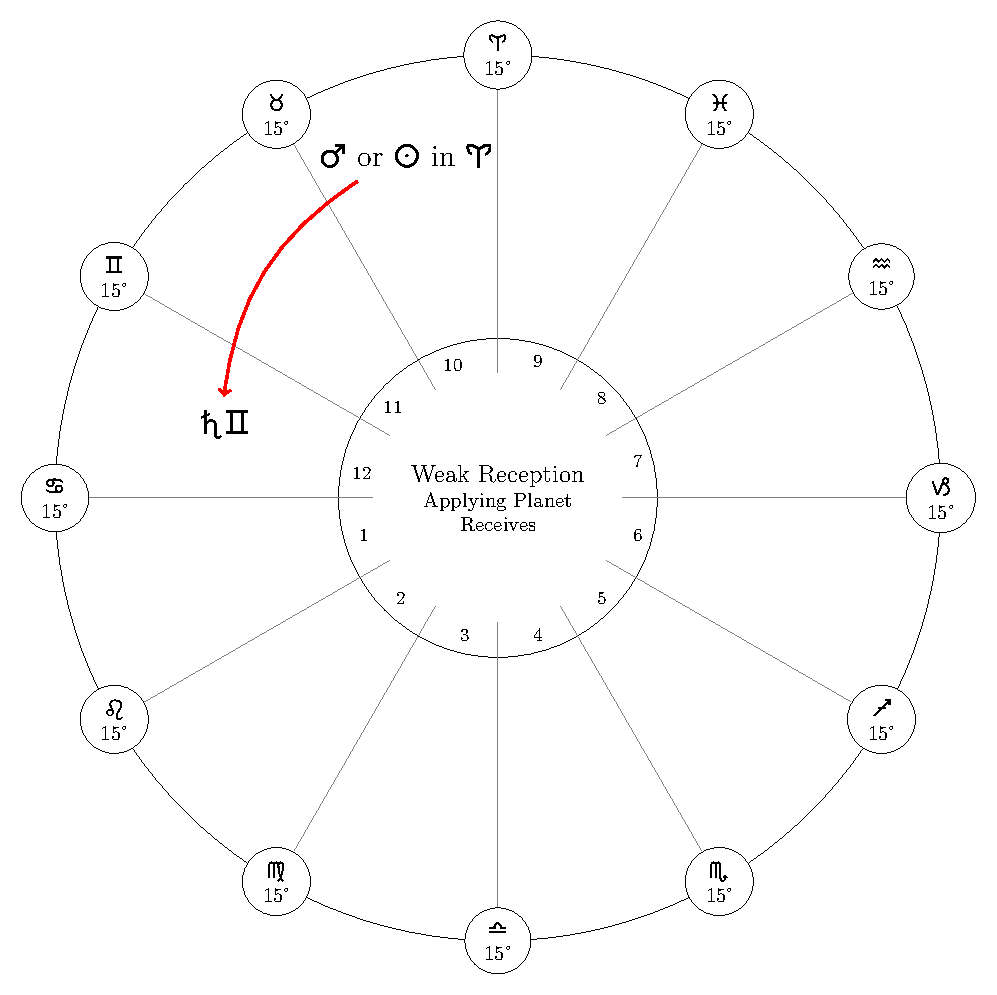
\includegraphics[width=\textwidth]{charts/01-weaker-reception}} \\
\end{center}

\end{columns}
\vspace{0.2cm}
\footnotetext[1]{Abu Ma'shar, p.25}
\footnotetext[2]{Ibn Ezra, p. 121}
\end{frame}
% ----------------------------------------------------
\begin{frame}[t]{What Constitues Reception - Pushing Nature}
\begin{columns}[T, onlytextwidth]
\column{0.5\textwidth}
\textbf{Example:} \Mars\ 10 \Aries\ $\Rightarrow$ \Conjunction\ \Saturn\ 15 \Aries\footnotemark[1] \\
\ul
\vspace{0.2cm}
\Mars\ is applying to \Conjunction\ \Saturn\ who is \Aries, therefore\\
\Mars\ \textsl{receives} \Saturn\ by domicile, but, \\
\Saturn\ does not receive \Mars\  \\

\vspace{0.2cm}
Ibn Ezra calls this \textsl{conferring of nature}, Abu Ma'shar, \textsl{pushing nature}; while according to Sahl, \Mars\ is \textsl{"giving [his] disposition and nature"} because he both rules and occupies \Aries; if he was in another sign he would only give his disposition (virtue) and not his nature.\footnotemark[2] \\

This can also happen if a planet is in its sign of exaltation and \Conjunction\ another planet in that same sign.


\column{0.5\textwidth}
\vspace{-0.5cm}
\begin{center}
{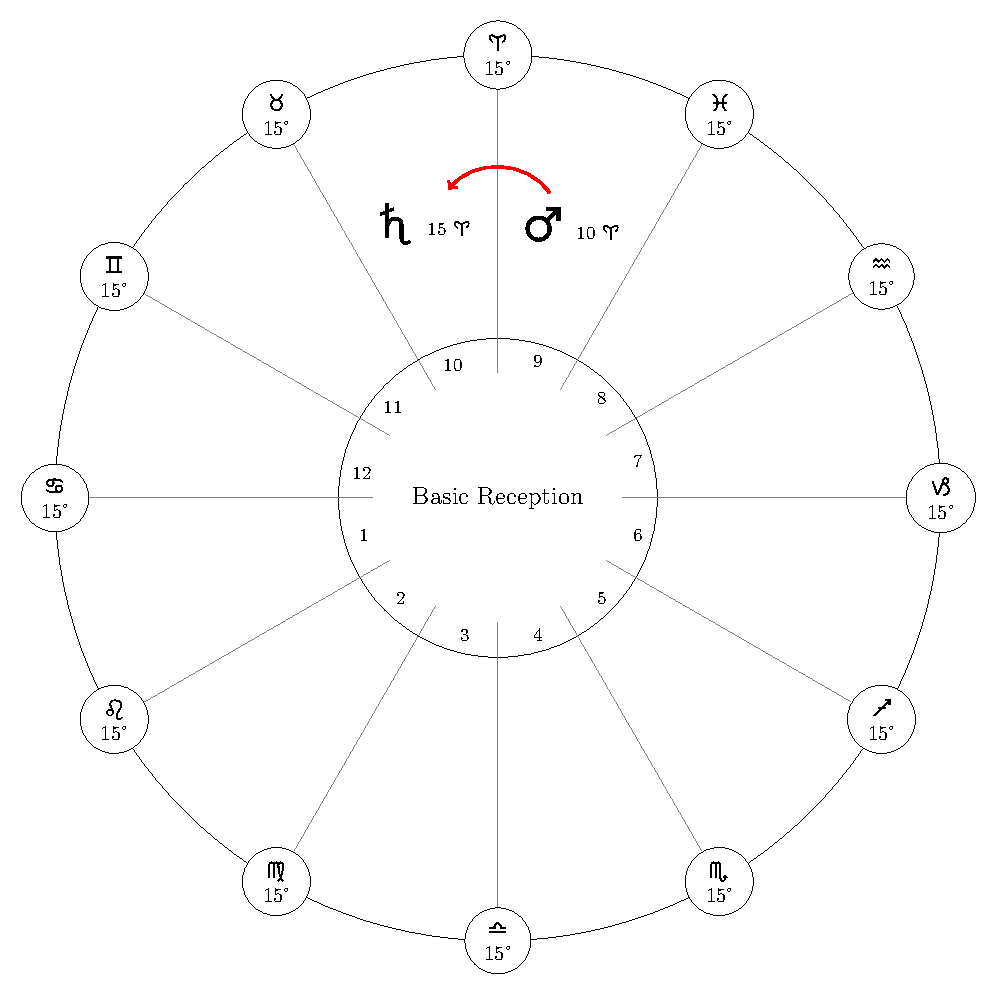
\includegraphics[width=0.9\textwidth]{charts/01-A-receives}} \\
\end{center}

\end{columns}
\vspace{0.2cm}
\footnotetext[1]{Masha'allah p.2}
\footnotetext[2]{Sahl, p.20-21}
\end{frame}
% ----------------------------------------------------
\begin{frame}[t]{What Constitutes Reception - Mutual Reception}
\begin{columns}[T, onlytextwidth]
\column{0.5\textwidth}
\textbf{Example:} \Mars\ 10 \Capricorn\ $\Rightarrow$ \Square\ \Saturn\ 20 \Aries \\
\ul
\vspace{0.5cm}
\Mars\ is in \Saturn's domicile (\Capricorn) applying to \Square\ \Saturn \\
\Saturn\ is in \Mars's domicile (\Aries), therefore, \\
\Mars\ receives \Saturn\ by domicile, and \\
\Saturn\ receives \Mars\ by domicile \\
\vspace{0.25cm}
giving  \textbf{Mutual Reception} [MR] by \textsl{domicile} \\
so \Mars\ receives \Saturn\ and commits his disposition to him and \Saturn\ receives it \\
\vspace{0.25cm}
This is the strongest form of reception; the second strongest form occurs when there is mutual reception by \textsl{exaltation}. i.e. both planets are in each other's sign of exaltation. i.e. \Venus\ in \Cancer\ \Trine\ \Jupiter\ in \Pisces.

\column{0.5\textwidth}

\begin{center}
{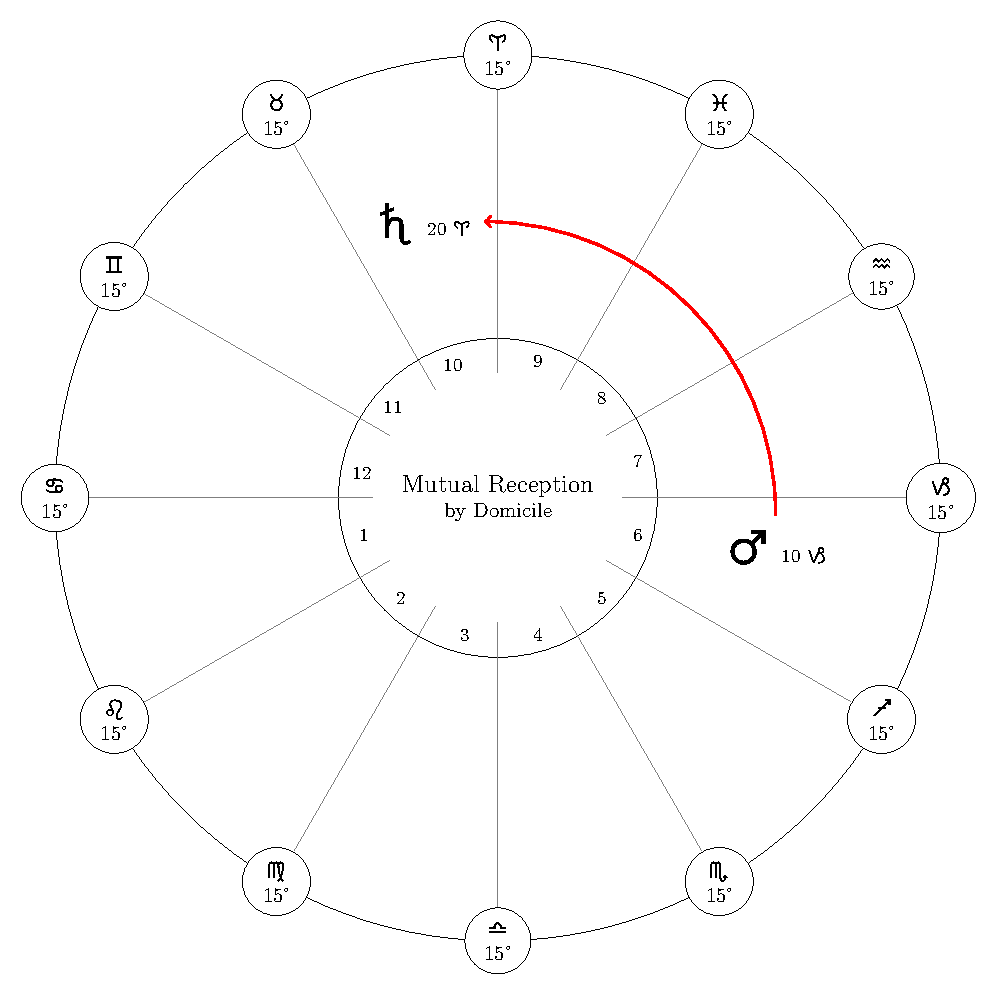
\includegraphics[width=0.9\textwidth]{charts/01-MR-by-domicile}} \\
\end{center}

\end{columns}
\end{frame}
% ----------------------------------------------------
\begin{frame}[t]{What Constitutes Reception - NOT Received}


\end{frame}
% ----------------------------------------------------
\begin{frame}[t]{What Constitutes Reception Continued}

Masha'allah tells us that if the matter being analyzed has to do with a King, the Exaltation rulers will have more authority over the matter than the domicile rulers.

As a general rule, reception is stronger if the planet applied to (usually the heavier planet) receives the applying planet (usually the lighter planet).

Later authors also considered reception by triplicity, term, and face but only considered it to be an \textsl{effective} reception if it involved at least two of these minor dignities i.e. received by triplicity and term or triplicity and face or term and face. Masha'allah does mention these minor dignities in his \textsl{Book of Thoughts and Intentions} but only in relation to determining which planet is stronger than another; he does not use them in any of his \textsl{On Reception} examples.

\end{frame}